%
% T�TULO DEL CAP�TULO
%
\chapter[Advanced GPU point rendering]{
	Advanced GPU point rendering
	\label{chapter_7}
}

The first approaches to point rendering like \cite{surfsplat} were CPU based, this was clearly not the right approach for real-time point rendering. To increase performance, the massively parallel computing power of GPUs should be taken advantage of. In a similar fashion to how triangle meshes are rendered nowadays, we will offload rendering to the graphics hardware freeing the CPU to perform other tasks. This will provide much higher performance than a CPU based solution. 

This would seem an easy task at first sight, but due to missing point splat support in graphics hardware; exploiting the GPU's hardware acceleration for point-based rendering is not an straightforward task. Fortunately, thanks to the introduction of fragment and vertex shaders, we will be able to use the hardware for this job using custom shaders.

\section[Performance details]{Performance details}

One of the reasons why point-based rendering is used, is the huge complexity of today's datasets (more than 1KM points), that can be acquired by LiDAR scanners. When these models are rendered, a triangle may only cover a few or not even one pixel. Since the triangle rasterization setup in this cases does not pay off, rendering massive triangle meshes is not efficient.

In these cases, is where points seem to be the more suited rendering primitive. But, when rendering massive point clouds, we should use the following guidelines:

\begin{itemize}
\item \textbf{Interleaved vertex arrays:} To minimize the number of calls to the OpenGL API, the point data (positions \textbf{p}, colors \textbf{c}, radii \textbf{r}, normals \textbf{n}, etc.) has to be stored in one large array. Thanks to this, we can render the points with just one call to \textit{glDrawArrays()}. For better memory coherence, the data should also be stored in an interleaved manner (i.e. $[\textbf{p}_{1},\textbf{p}_{2},\ldots,\textbf{c}_{1},\textbf{c}_{2},\ldots]$).
\item \textbf{Vertex Buffer Objects:} In each frame, all the point data has to be transferred to the GPU. This would quickly become a bottleneck in massive datasets. Since sometimes this data will be static for several frames, it will be stored in high performance video memory for efficient GPU access. VBOs are the standard way of achieving our objective since OpenGL version 1.5 (2003).
\item \textbf{Data formats:} In order to reduce the GPU memory consumed, and decrease transfer costs, the point data will be stored in a compact format. Position and normals will be stored using single-precision floating-point numbers, colors will be stored using just 4 bytes (one per RGBA channel). 
\item \textbf{Shading language:} Low-level shading languages offer a small performance advantage, but since nowadays it is marginal, GLSL will be used for shader programming. High-level languages like GLSL are more convenient to use and way less problematic when adding features or reviewing the code.
\end{itemize} 

TODO optimum VBO size

All of these optimization techniques are valid for all the point rendering approaches that will be explained next. 

\section[Splat rasterization]{Splat rasterization}

This is the first step in splat rendering, it determines the pixels that a point will cover. Since there are no splat primitives, splats have to be created from other rendering primitives, like points or triangles. All of the following methods were implemented and tested in modern OpenGL, the code can be reviewed in the repository of the project (\url{http://tovias.citic.udc.es/}). 

\subsection[Image-aligned squares]{Image-aligned squares}

For the highest performance, splats should be rendered using only one OpenGL point for each splat, using:
\\
\lstset{emph={[2]glDrawArrays}, emphstyle={[2]\color{PineGreen}},emph={[3]GL_POINTS}, emphstyle={[3]\color{RawSienna}}}
\begin{lstlisting}
 glDrawArrays(GL_POINTS, 0, VBOSize);
\end{lstlisting}

An optional output of a vertex shader is the point size, that when set to $s$, creates a image-space square of $s \times s$ pixels centered in the vertex position. Instead of squares, image aligned circles can be rendered by enabling point smoothing and MSAA:
\\
\lstset{emph={[2]glEnable}, emphstyle={[2]\color{PineGreen}},emph={[3]GL_POINT_SMOOTH}, emphstyle={[3]\color{RawSienna}}}
\begin{lstlisting}
 glEnable(GL_POINT_SMOOTH);
\end{lstlisting}

TODO simple way without msaa in fragment

The screen-space size of the projected OpenGL point has to be adjusted in the vertex shader, so that holes do not appear when moving closer to the object. To allow us to modify the point size dynamically in the vertex shader and specify our coordinate system origin, we will use the following code:
\\
\lstset{emph={[2]glEnable,glPointParameteri}, emphstyle={[2]\color{PineGreen}},emph={[3]GL_PROGRAM_POINT_SIZE,GL_POINT_SPRITE_COORD_ORIGIN,GL_LOWER_LEFT}, 
		emphstyle={[3]\color{RawSienna}}}
\begin{lstlisting}
 glEnable(GL_PROGRAM_POINT_SIZE);
 glPointParameteri(GL_POINT_SPRITE_COORD_ORIGIN, GL_LOWER_LEFT);
\end{lstlisting}

The adjusted point size is approximated by calculating the foreshortening of the point radii $r$, depending on the point position $\mathbf{p}$ in camera coordinates:

\begin{equation} s = 1.5\cdot r\cdot \frac{n}{p_{z}}\cdot \frac{h}{t-b} \end{equation}

Where $n$, $t$ and $b$ are the near/top/bottom parameters of the camera's view frustum and $h$ the height of the viewport in pixels. The advantage of this rasterization method, is that because of its simplicity, it is the fastest of the three studied methods. It is also the one that requires the least amount of information, since it only needs the splat position, color and optionally radius. 

\begin{figure}[h]
	\centering
	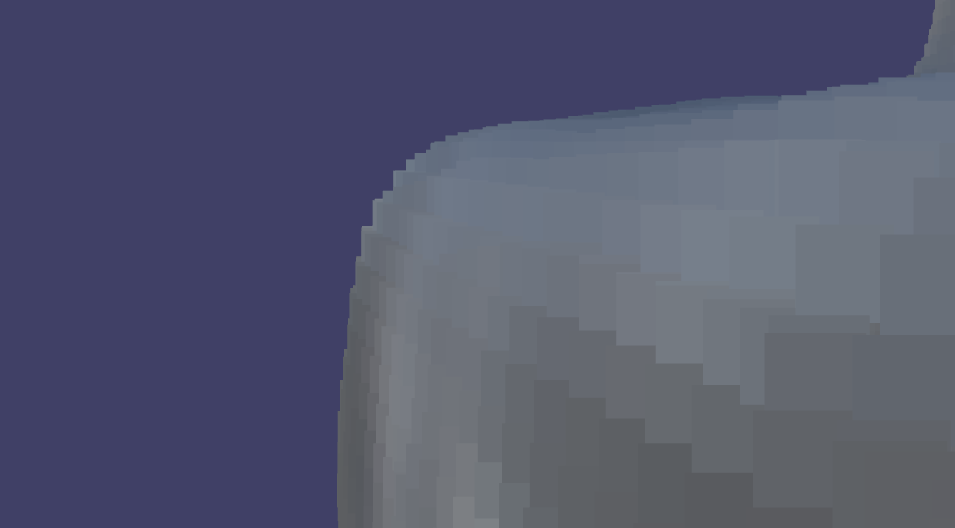
\includegraphics[scale=0.5]{figures/squares.png}
	\caption[Image aligned square defects]{
		Render image showing the defects that image-aligned squares present in object contours.
	}
	\label{squares}
\end{figure}

However, this method is not optimal for high quality rendering. It yields bad results specially near the object's contour (see \autoref{squares}), where the poor approximation of the splat shape is specially noticeable. Furthermore, since all fragments created with this technique have the same depth value, this prevents the correct blending of overlapping splats.

\subsection[Affinely projected point sprites]{Affinely projected point sprites}

An improved approximation to the true splat shape is the one in \cite{circularsplats}, this technique was called circular object-space splats. It starts by adjusting the point size in the vertex shader as in the previous method, but for each of the squares, the fragment shader will determine whether or not the fragment corresponds to the inside or outside of the splat. 

Fragments outside the splat will be discarded using the \textit{discard} GLSL command. This will result in circular splat rasterization. For this technique to work we will have to activate the following feature in OpenGL:
\\
\lstset{emph={[2]glEnable}, emphstyle={[2]\color{PineGreen}},emph={[3]GL_POINT_SPRITE}, 
		emphstyle={[3]\color{RawSienna}}}
\begin{lstlisting}
 glEnable(GL_POINT_SPRITE);
\end{lstlisting} 

Next, we need to parameterize the screen-space square in the range $[-r,r]^2$, being $r$ the splat radius. For each of its fragments $(x,y) \in [-r,r]^2$, a depth offset $\delta z$ from the splat center $\mathbf{p}$ can be computed as a linear function that depends on the camera-space normal vector $\mathbf{n} = (n_{x},n_{y},n_{z})$:

\begin{equation}\label{eq:depth} \delta z = -\frac{n_{x}}{n_{z}} \cdot x - \frac{n_{y}}{n_{z}} \cdot y \end{equation}

The depth offset can after this step be used to compute the 3D distance to the splat center. This distance can then be used to check whether a the fragment corresponds to the inside of the splat or not with:

\begin{equation} \left \| (x,y,\delta z) \right \| \leq r \end{equation}

Since one of the problems that we found in the image-aligned squares was the lack of a depth value for the splat, the depth offset $\delta z$ should also be used to correct the fragment's depth value. Starting from the camera space depth value $z' = p_{z} + \delta z$, the frustum and viewport transformations allow us to calculate the window-space depth buffer entry, from the far plane $f$ and the near plane $n$:

\begin{equation}\label{eq:zbuffer} \text{zbuffer}(x,y) = \frac{1}{z'} \cdot \frac{fn}{f-n} \cdot \frac{f}{f-n} \end{equation} 

This approach yields much better results in comparison to the previous one, this is specially apparent in object contours. But it does not come without its share of issues. Since the depth offset is just an approximation due to the fact that in the \autoref{eq:depth} a parallel projection is assumed. Thus neglecting the angle between the viewing ray and the splat normal. This creates artifacts when viewing the splat from extreme angles (see \autoref{ext_angles}).



\subsection[Perspectively correct rasterization]{Perspectively correct rasterization}

The last approximation was able to correctly transform the splat center, but failed to do the same with the contour, this caused holes to appear in the rendered image. This is why, to create a perspective correct approximation, the technique in \cite{perspcorrect} was created. In this method, the outer contour of the splat was correctly transformed, but had projective errors in the splat center. This approach had a high computational cost, that made it very costly.

\begin{figure}[h]
	\centering
	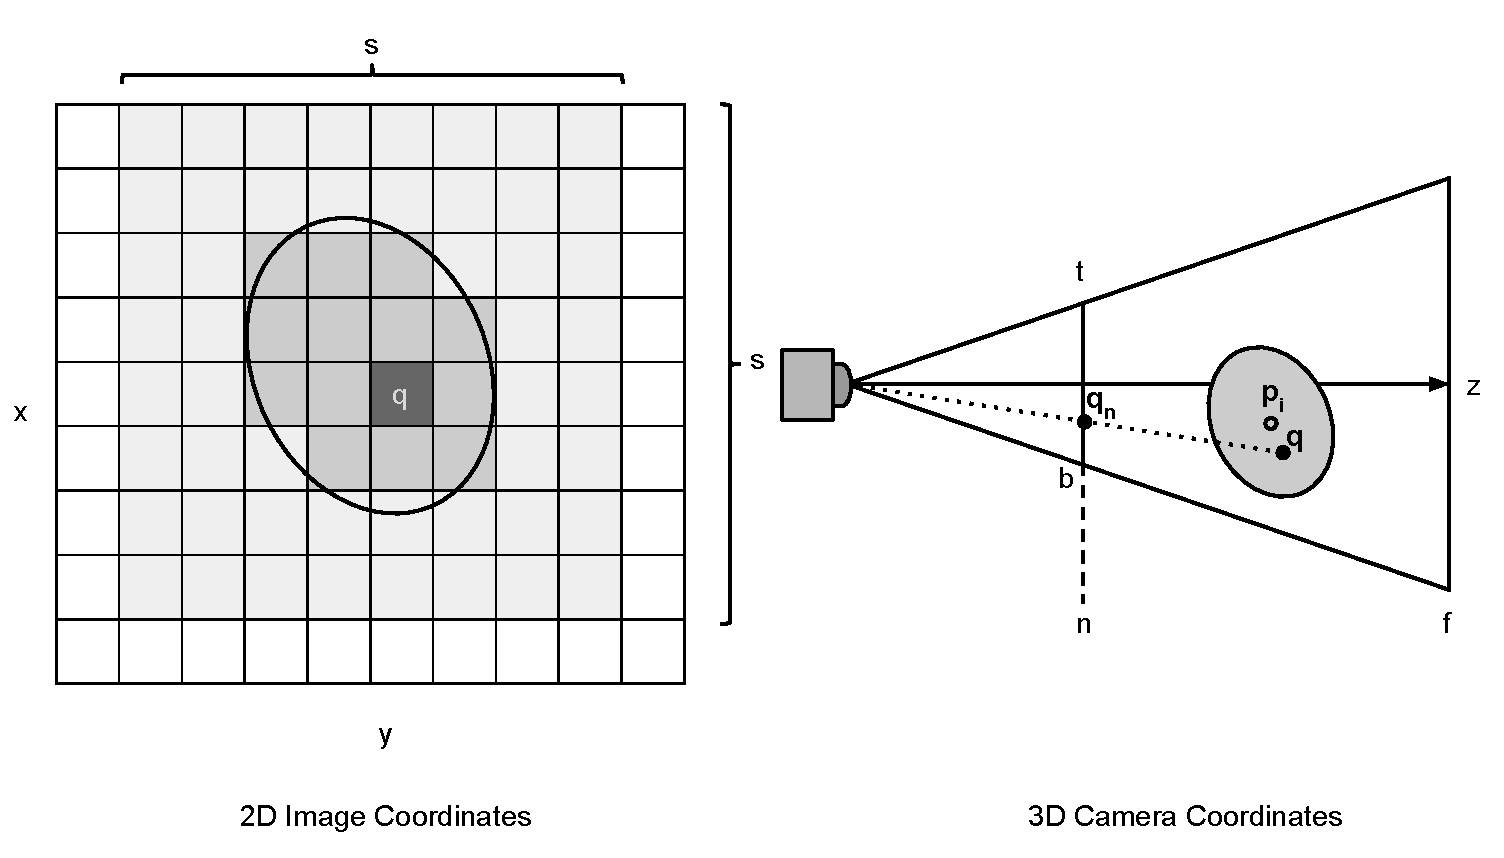
\includegraphics[scale=0.5]{figures/persp_accu.pdf}
	\caption[Perspective accurate]{
		Projection of the splat and raycasting visual explanation.
	}
	\label{persp_accu}
\end{figure}

A more efficient while being perspective correct technique was presented in \cite{perspeffi}. The main concept in this method is to determine the 3D point corresponding to a 2D fragment based on local raycasting. This method can also handle elliptical splats, although we will concentrate our efforts in circular splats since this is our case study.

A splat $s_{i}$ is represented by a center $\mathbf{p_{i}}$, a radius $r_{i}$ and its normal $\mathbf{n_{i}}$. We start by rendering the splats again with \textit{GL\_POINTS} and the pixel size given by the splat radius. Next, for each fragment $(x,y)$ the \textit{exact} corresponding 3D point $\mathbf{q}$ is computed using local raycasting (see \autoref{persp_accu}). With this point $\mathbf{q}$, the distance to the center of the splat is computed, if the fragment lies outside of the splat it is discarded with the \textit{discard} command. The \autoref{eq:dist} dictates if the fragment is outside or inside the splat:

\begin{equation}\label{eq:dist} \left \| \mathbf{q} - \mathbf{p_{i}} \right \| \leq r \end{equation} 

To compute $\mathbf{q}$ we will first need to invert the window-to-viewport transformation, mapping the fragment $(x,y)$ to a 3D point $\mathbf{q_{n}}$ on the near plane:

\begin{equation} 
\mathbf{q_{n}} = 
\begin{pmatrix}
x\cdot \frac{r-l}{w}-\frac{r-l}{2}
\\
y\cdot \frac{t-b}{h}-\frac{t-b}{2}
\\ 
-n
\end{pmatrix} 
\end{equation}  

Being $b$/$t$/$l$/$r$ the bottom/top/left/right corners of the frustum and $w$/$h$ the width/height of the viewport. Casting a ray from the origin through the point $\mathbf{q_{n}}$ and intersecting with the splats supporting plane will yield the necessary point $\mathbf{q}$. First we will calculate the distance at which the ray intersects the plane:

\begin{equation} t = \frac{\mathbf{p_{i}} \cdot \mathbf{n_{i}}}{\mathbf{q_{n} \cdot \mathbf{n_{i}}}} \end{equation}  

Once the distance $t$ is obtained, the point $\mathbf{q}$ is easily obtained with the following equation:

\begin{equation} \mathbf{q} = t\mathbf{q_{n}} \end{equation}  

After the point $\mathbf{q}$ is known, we can apply \autoref{eq:dist} to test whether the fragment falls inside the splat or not. Of course, we will not be done until we adjust the new fragment depth value using $q_{z}$ as $z'$ in \autoref{eq:zbuffer}. Since the 3D point $\mathbf{q}$ is the \textit{exact} preimage of the projective transform, this means that this method is perspectively correct for each pixel.    

\section[Antialiasing]{Antialiasing}
